% Power BI Automated Validation Framework -- Architecture wireframe
%
% Compile with: pdflatex architecture_wireframe.tex   (or open in Overleaf)
% Not compiled/verified locally -- no LaTeX install on the machine this was
% authored on. Layout uses absolute `at (x,y)` coordinates throughout (not
% chained relative positioning) specifically to minimize alignment risk that
% can't be visually caught without a compiler. If anything overlaps or looks
% off once you compile it, the coordinates are easy to nudge -- see the
% "LAYOUT GRID" comment block below for the column/row scheme.
%
% Solid arrows = live pytest call path. Dashed arrows = blocked/optional/
% offline path.

\documentclass[tikz,border=14pt]{standalone}
\usepackage{tikz}
\usetikzlibrary{positioning, arrows.meta, fit, backgrounds}

\begin{document}
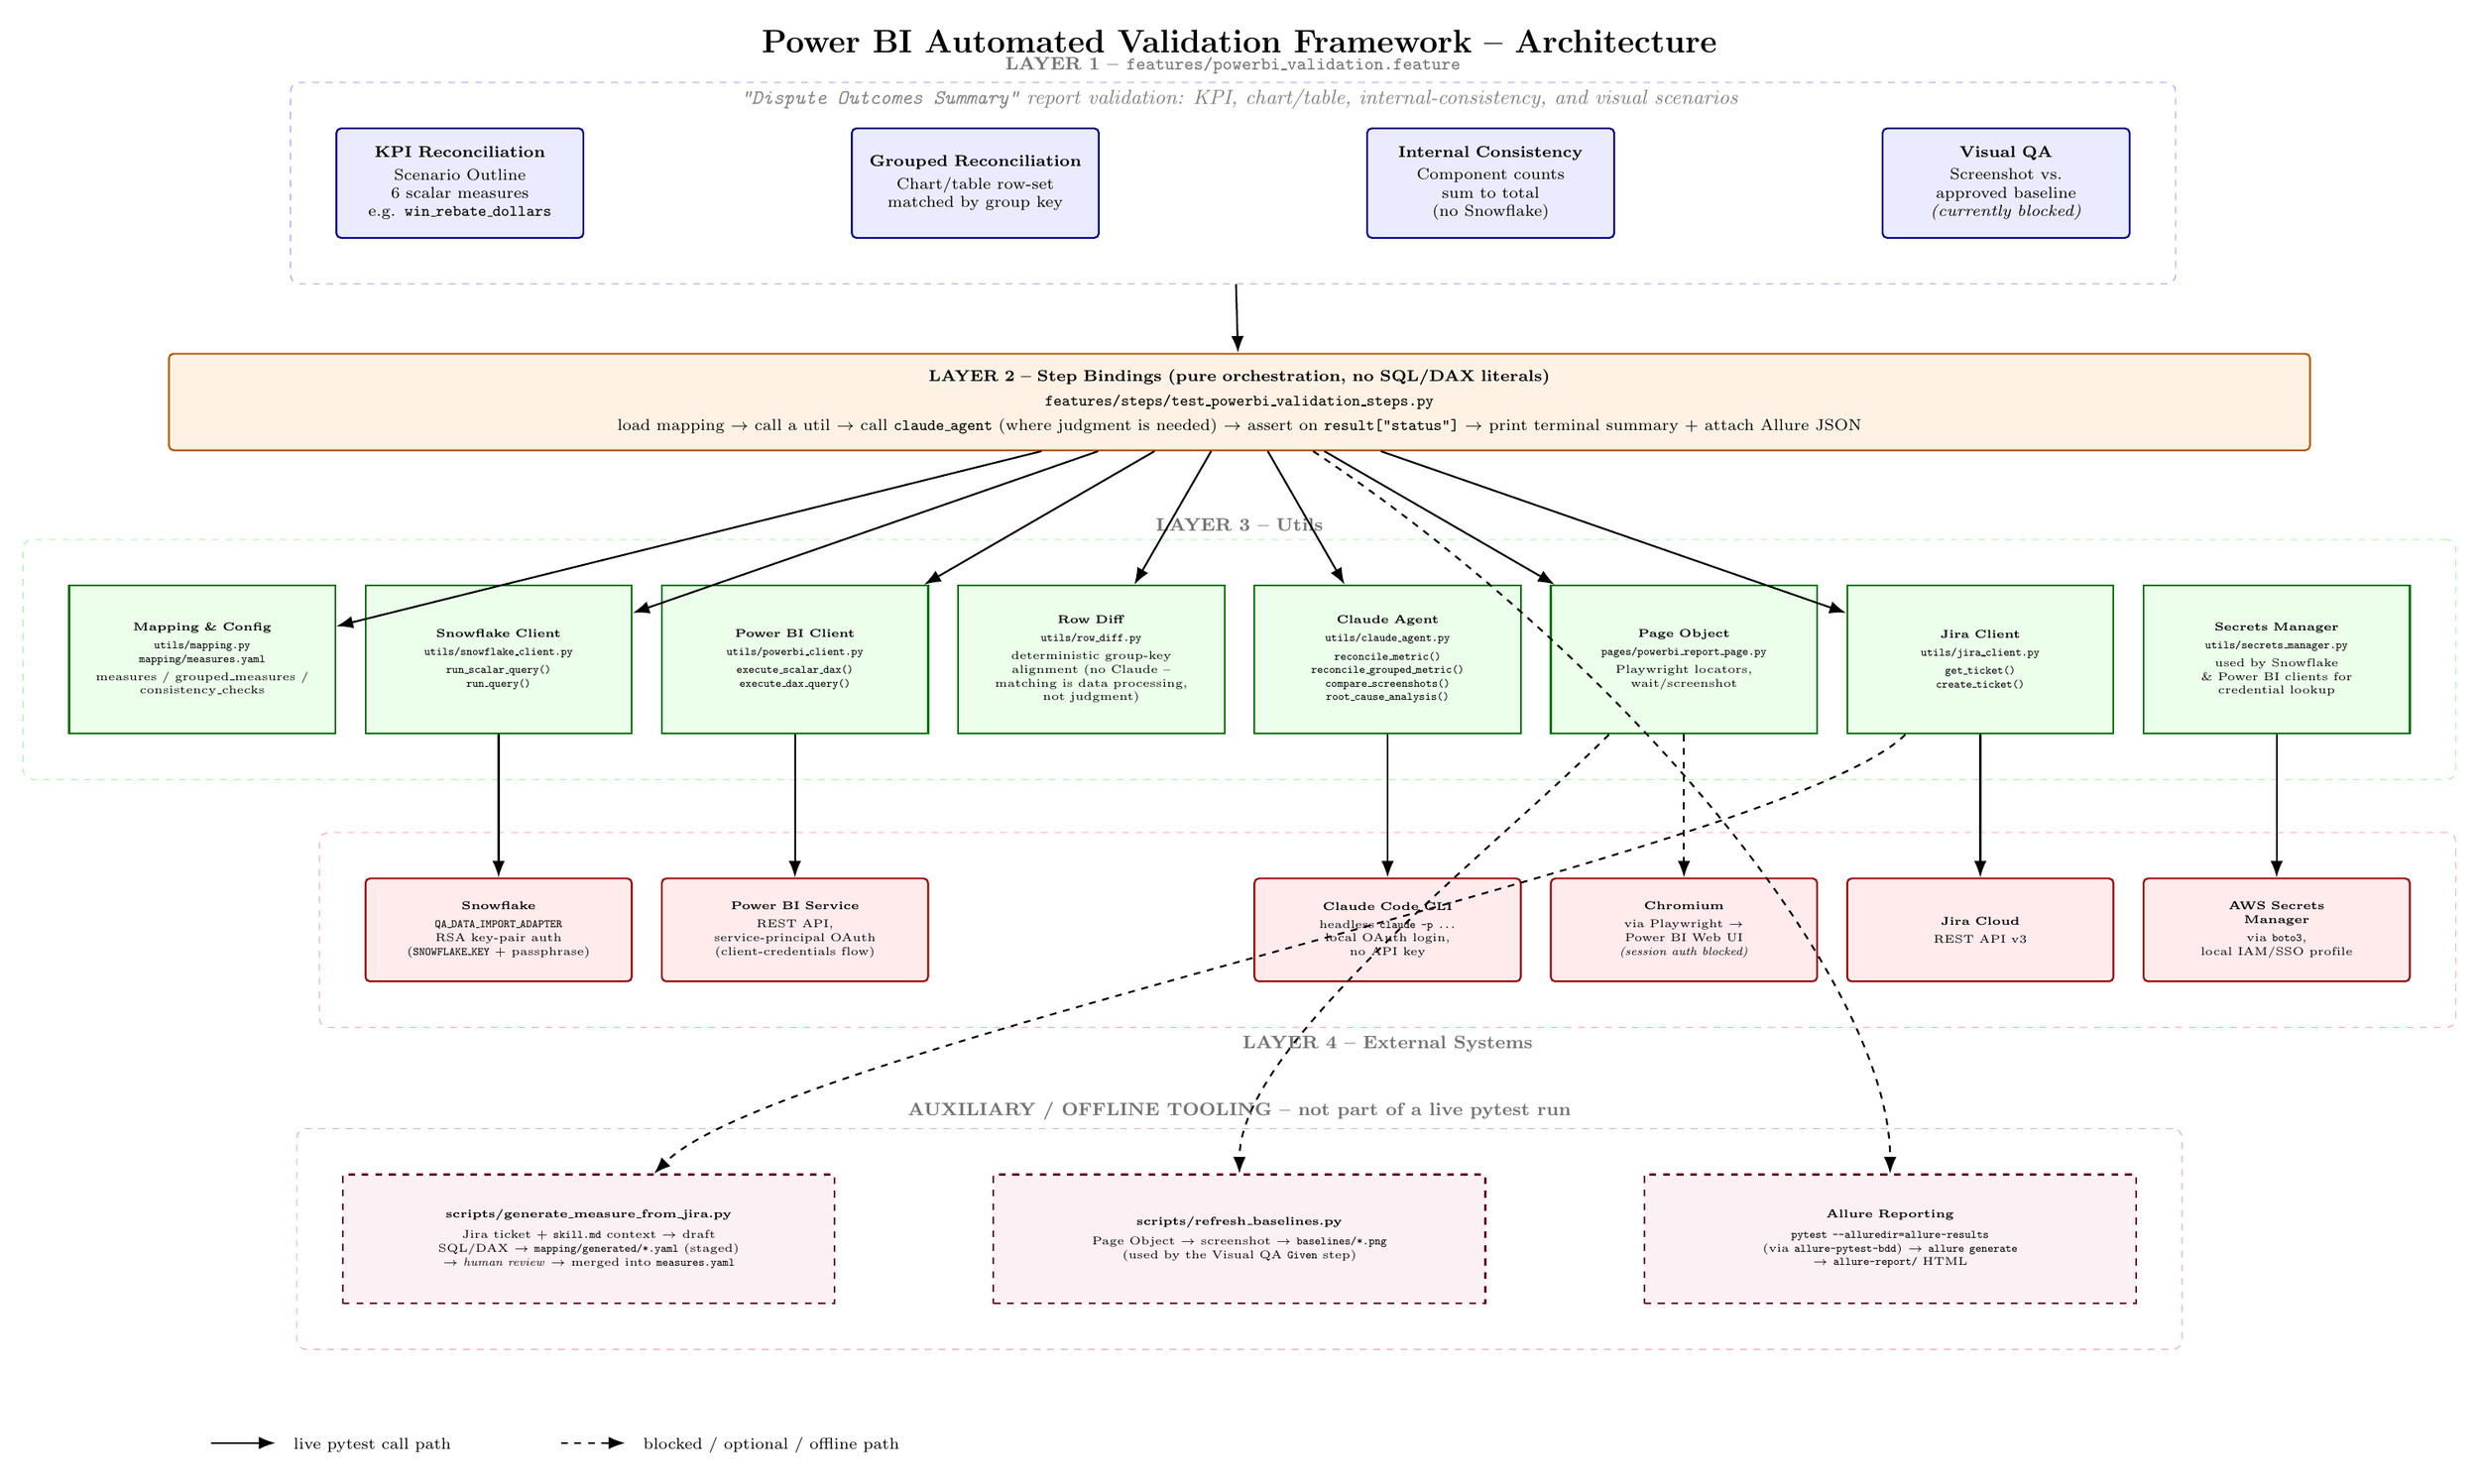
\begin{tikzpicture}[
  font=\sffamily,
  every node/.style={align=center},
  scenario/.style={rectangle, rounded corners=2pt, draw=blue!55!black, thick,
    fill=blue!8, text width=3.6cm, minimum height=1.7cm, font=\scriptsize},
  orchestration/.style={rectangle, rounded corners=2pt, draw=orange!70!black,
    thick, fill=orange!10, text width=33cm, minimum height=1.5cm, font=\scriptsize},
  util/.style={rectangle, draw=green!45!black, thick, fill=green!8,
    text width=3.9cm, minimum height=2.3cm, font=\tiny},
  external/.style={rectangle, rounded corners=2pt, draw=red!60!black, thick,
    fill=red!8, text width=3.9cm, minimum height=1.6cm, font=\tiny},
  tool/.style={rectangle, dashed, draw=purple!55!black, thick, fill=purple!6,
    text width=7.4cm, minimum height=2cm, font=\tiny},
  flow/.style={-{Latex[length=2.6mm]}, thick},
  optflow/.style={-{Latex[length=2.6mm]}, thick, dashed},
  layerlabel/.style={font=\bfseries\footnotesize, text=black!55}
]

% =====================================================================
% LAYOUT GRID (cm): 8 columns at x = 0,4.6,9.2,13.8,18.4,23.0,27.6,32.2
% Rows (y, top to bottom): 0 (Gherkin) / -3.4 (Orchestration) /
% -7.4 (Utils) / -11.6 (External systems) / -16.4 (Auxiliary tooling)
% =====================================================================

% Title
\node[font=\bfseries\Large] at (16.1, 2.2)
  {Power BI Automated Validation Framework -- Architecture};
\node[font=\itshape\small, text=black!50] at (16.1, 1.3)
  {\texttt{"Dispute Outcomes Summary"} report validation: KPI, chart/table,
   internal-consistency, and visual scenarios};

% ---------------------------------------------------------------------
% ROW 1 -- Gherkin (business-readable, no logic)
% ---------------------------------------------------------------------
\node[scenario] (s1) at (4, 0)
  {\textbf{KPI Reconciliation}\\[2pt]Scenario Outline\\6 scalar measures\\
   e.g. \texttt{win\_rebate\_dollars}};
\node[scenario] (s2) at (12, 0)
  {\textbf{Grouped Reconciliation}\\[2pt]Chart/table row-set\\
   matched by group key};
\node[scenario] (s3) at (20, 0)
  {\textbf{Internal Consistency}\\[2pt]Component counts\\
   sum to total\\(no Snowflake)};
\node[scenario] (s4) at (28, 0)
  {\textbf{Visual QA}\\[2pt]Screenshot vs.\\approved baseline\\
   \textit{(currently blocked)}};

\begin{scope}[on background layer]
\node[fit=(s1)(s2)(s3)(s4), inner sep=7mm, draw=blue!40, dashed,
  rounded corners=4pt,
  label={[layerlabel]above:LAYER 1 -- \texttt{features/powerbi\_validation.feature}}]
  (layer1) {};
\end{scope}

% ---------------------------------------------------------------------
% ROW 2 -- Orchestration
% ---------------------------------------------------------------------
\node[orchestration] (steps) at (16.1, -3.4)
  {\textbf{LAYER 2 -- Step Bindings (pure orchestration, no SQL/DAX literals)}\\[3pt]
   \texttt{features/steps/test\_powerbi\_validation\_steps.py}\\[3pt]
   load mapping $\rightarrow$ call a util $\rightarrow$ call \texttt{claude\_agent}
   (where judgment is needed) $\rightarrow$ assert on \texttt{result["status"]}
   $\rightarrow$ print terminal summary + attach Allure JSON};

\draw[flow] (layer1) -- (steps);

% ---------------------------------------------------------------------
% ROW 3 -- Utils (thick layer: config, data access, judgment, determinism)
% ---------------------------------------------------------------------
\node[util] (mapping) at (0, -7.4)
  {\textbf{Mapping \& Config}\\[2pt]\texttt{utils/mapping.py}\\
   \texttt{mapping/measures.yaml}\\[2pt]
   measures / grouped\_measures /\\consistency\_checks};
\node[util] (sfclient) at (4.6, -7.4)
  {\textbf{Snowflake Client}\\[2pt]\texttt{utils/snowflake\_client.py}\\[2pt]
   \texttt{run\_scalar\_query()}\\\texttt{run\_query()}};
\node[util] (pbiclient) at (9.2, -7.4)
  {\textbf{Power BI Client}\\[2pt]\texttt{utils/powerbi\_client.py}\\[2pt]
   \texttt{execute\_scalar\_dax()}\\\texttt{execute\_dax\_query()}};
\node[util] (rowdiff) at (13.8, -7.4)
  {\textbf{Row Diff}\\[2pt]\texttt{utils/row\_diff.py}\\[2pt]
   deterministic group-key\\alignment (no Claude --\\
   matching is data processing,\\not judgment)};
\node[util] (claudeagent) at (18.4, -7.4)
  {\textbf{Claude Agent}\\[2pt]\texttt{utils/claude\_agent.py}\\[2pt]
   \texttt{reconcile\_metric()}\\\texttt{reconcile\_grouped\_metric()}\\
   \texttt{compare\_screenshots()}\\\texttt{root\_cause\_analysis()}};
\node[util] (pageobj) at (23.0, -7.4)
  {\textbf{Page Object}\\[2pt]\texttt{pages/powerbi\_report\_page.py}\\[2pt]
   Playwright locators,\\wait/screenshot};
\node[util] (jiraclient) at (27.6, -7.4)
  {\textbf{Jira Client}\\[2pt]\texttt{utils/jira\_client.py}\\[2pt]
   \texttt{get\_ticket()}\\\texttt{create\_ticket()}};
\node[util] (secrets) at (32.2, -7.4)
  {\textbf{Secrets Manager}\\[2pt]\texttt{utils/secrets\_manager.py}\\[2pt]
   used by Snowflake \\\& Power BI clients for\\credential lookup};

\begin{scope}[on background layer]
\node[fit=(mapping)(sfclient)(pbiclient)(rowdiff)(claudeagent)(pageobj)(jiraclient)(secrets),
  inner sep=7mm, draw=green!40, dashed, rounded corners=4pt,
  label={[layerlabel]above:LAYER 3 -- Utils}] (layer3) {};
\end{scope}

\draw[flow] (steps) -- (mapping);
\draw[flow] (steps) -- (sfclient);
\draw[flow] (steps) -- (pbiclient);
\draw[flow] (steps) -- (rowdiff);
\draw[flow] (steps) -- (claudeagent);
\draw[flow] (steps) -- (pageobj);
\draw[flow] (steps) -- (jiraclient);

% ---------------------------------------------------------------------
% ROW 4 -- External systems (only where a util actually reaches outside)
% ---------------------------------------------------------------------
\node[external] (sfdb) at (4.6, -11.6)
  {\textbf{Snowflake}\\[2pt]\texttt{QA\_DATA\_IMPORT\_ADAPTER}\\
   RSA key-pair auth\\(\texttt{SNOWFLAKE\_KEY} + passphrase)};
\node[external] (pbisvc) at (9.2, -11.6)
  {\textbf{Power BI Service}\\[2pt]REST API,\\
   service-principal OAuth\\(client-credentials flow)};
\node[external] (claudecli) at (18.4, -11.6)
  {\textbf{Claude Code CLI}\\[2pt]headless \texttt{claude -p ...}\\
   local OAuth login,\\no API key};
\node[external] (chromium) at (23.0, -11.6)
  {\textbf{Chromium}\\[2pt]via Playwright $\rightarrow$\\
   Power BI Web UI\\\textit{(session auth blocked)}};
\node[external] (jiracloud) at (27.6, -11.6)
  {\textbf{Jira Cloud}\\[2pt]REST API v3};
\node[external] (awssecrets) at (32.2, -11.6)
  {\textbf{AWS Secrets}\\\textbf{Manager}\\[2pt]via \texttt{boto3},\\
   local IAM/SSO profile};

\begin{scope}[on background layer]
\node[fit=(sfdb)(pbisvc)(claudecli)(chromium)(jiracloud)(awssecrets),
  inner sep=7mm, draw=red!35, dashed, rounded corners=4pt,
  label={[layerlabel]below:LAYER 4 -- External Systems}] (layer4) {};
\end{scope}

\draw[flow] (sfclient) -- (sfdb);
\draw[flow] (pbiclient) -- (pbisvc);
\draw[flow] (claudeagent) -- (claudecli);
\draw[optflow] (pageobj) -- (chromium);
\draw[flow] (jiraclient) -- (jiracloud);
\draw[flow] (secrets) -- (awssecrets);

% ---------------------------------------------------------------------
% AUXILIARY / OFFLINE TOOLING -- not part of a live pytest run
% ---------------------------------------------------------------------
\node[tool] (jiragen) at (6, -16.4)
  {\textbf{scripts/generate\_measure\_from\_jira.py}\\[3pt]
   Jira ticket + \texttt{skill.md} context $\rightarrow$ draft SQL/DAX
   $\rightarrow$ \texttt{mapping/generated/*.yaml} (staged) $\rightarrow$
   \textit{human review} $\rightarrow$ merged into \texttt{measures.yaml}};
\node[tool] (baselines) at (16.1, -16.4)
  {\textbf{scripts/refresh\_baselines.py}\\[3pt]
   Page Object $\rightarrow$ screenshot $\rightarrow$
   \texttt{baselines/*.png}\\(used by the Visual QA \texttt{Given} step)};
\node[tool] (allure) at (26.2, -16.4)
  {\textbf{Allure Reporting}\\[3pt]
   \texttt{pytest --alluredir=allure-results}\\(via \texttt{allure-pytest-bdd})
   $\rightarrow$ \texttt{allure generate}\\$\rightarrow$ \texttt{allure-report/} HTML};

\begin{scope}[on background layer]
\node[fit=(jiragen)(baselines)(allure), inner sep=7mm, draw=purple!35, dashed,
  rounded corners=4pt,
  label={[layerlabel]above:AUXILIARY / OFFLINE TOOLING -- not part of a live pytest run}]
  (layer5) {};
\end{scope}

\draw[optflow] (jiraclient) .. controls +(-3,-3) and +(3,3) .. (jiragen);
\draw[optflow] (pageobj) .. controls +(-3,-3) and +(0,3) .. (baselines);
\draw[optflow] (steps) .. controls +(6,-4) and +(0,4) .. (allure);

% ---------------------------------------------------------------------
% Legend
% ---------------------------------------------------------------------
% NOTE: a nested \tikz{...} here would NOT inherit the outer picture's named
% styles (flow/optflow are scoped to this tikzpicture instance) -- so the
% arrow styles are written out explicitly instead of by name.
\node[anchor=west, font=\scriptsize] at (0, -19.6)
  {\tikz{\draw[-{Latex[length=2.6mm]}, thick] (0,0) -- (1,0);} \; live pytest call path
   \hspace{1.5cm}
   \tikz{\draw[-{Latex[length=2.6mm]}, thick, dashed] (0,0) -- (1,0);} \; blocked / optional / offline path};

\end{tikzpicture}
\end{document}
